\documentclass{article}
\usepackage{tikz}
\usetikzlibrary{arrows.meta}

% --- Custom Cubing Styles ---
\tikzset{
    % Top face stickers (Always Yellow for PLL)
    top-y/.style={fill=yellow!95!black, draw=black, thick},
    % Adjacent side colors (Standard scheme: Green, Red, Blue, Orange)
    side-G/.style={fill=green!70!black, draw=black, thick},
    side-R/.style={fill=red!80!black, draw=black, thick},
    side-B/.style={fill=blue!70!black, draw=black, thick},
    side-O/.style={fill=orange!90!black, draw=black, thick},
    % Movement arrows
    pllarrow/.style={thick, -{Stealth[scale=1.3]}, red, line width=1.5pt}
}

\begin{document}
\section*{PLL Diagrams}

\hfill

% ==================== CASE 1: Ub PERM ====================
\begin{minipage}{0.45\textwidth}
\centering
\subsubsection*{Ub-Permutation}
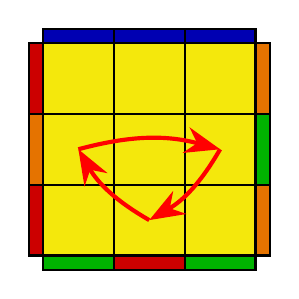
\begin{tikzpicture}[scale=0.9]
    % --- 1. Top Yellow Face (Solved) ---
    \foreach \x in {0,1,2} {
        \foreach \y in {0,1,2} {
            \path[top-y] (\x,\y) rectangle (\x+1,\y+1);
        }
    }

    % --- 2. Adjacent Side Stickers (Outer Ring) ---
    % BACK (Top edge of diagram - Blue face)
    \path[side-B] (0,3) rectangle (1,3.2);
    \path[side-B] (1,3) rectangle (2,3.2);
    \path[side-B] (2,3) rectangle (3,3.2);
    
    % FRONT (Bottom edge of diagram - Green face)
    \path[side-G] (0,-0.2) rectangle (1,0);
    \path[side-R] (1,-0.2) rectangle (2,0); % Scrambled Edge (Red)
    \path[side-G] (2,-0.2) rectangle (3,0);
    
    % LEFT (Left edge of diagram - Orange face)
    \path[side-R] (-0.2,0) rectangle (0,1);
    \path[side-O] (-0.2,1) rectangle (0,2); % Scrambled Edge (Green)
    \path[side-R] (-0.2,2) rectangle (0,3);
    
    % RIGHT (Right edge of diagram - Red face)
    \path[side-O] (3,0) rectangle (3.2,1);
    \path[side-G] (3,1) rectangle (3.2,2); % Scrambled Edge (Orange)
    \path[side-O] (3,2) rectangle (3.2,3);

    % --- 3. Permutation Arrows ---
    % Cycles edges: Front -> Left -> Right
    \draw[pllarrow] (1.5, 0.5) to[bend left=15] (0.5, 1.5);
    \draw[pllarrow] (0.5, 1.5) to[bend left=15] (2.5, 1.5);
    \draw[pllarrow] (2.5, 1.5) to[bend left=15] (1.5, 0.5);
    
\end{tikzpicture}

\medskip
\texttt{R2 U (R U R' U') R' U' (R' U R')}
\end{minipage}
\hfill
% ==================== CASE 2: Ua PERM ====================
\begin{minipage}{0.45\textwidth}
\centering
\subsubsection*{Ua-Permutation}
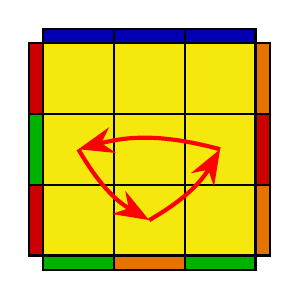
\begin{tikzpicture}[scale=0.9]
    % --- 1. Top Yellow Face (Solved) ---
    \foreach \x in {0,1,2} {
        \foreach \y in {0,1,2} {
            \path[top-y] (\x,\y) rectangle (\x+1,\y+1);
        }
    }

    % --- 2. Adjacent Side Stickers (Outer Ring) ---
    % BACK
    \path[side-B] (0,3) rectangle (1,3.2);
    \path[side-B] (1,3) rectangle (2,3.2);
    \path[side-B] (2,3) rectangle (3,3.2);
    
    % FRONT
    \path[side-G] (0,-0.2) rectangle (1,0); % Scrambled Corner (Orange)
    \path[side-O] (1,-0.2) rectangle (2,0);
    \path[side-G] (2,-0.2) rectangle (3,0);
    
    % LEFT
    \path[side-R] (-0.2,0) rectangle (0,1);
    \path[side-G] (-0.2,1) rectangle (0,2);
    \path[side-R] (-0.2,2) rectangle (0,3); % Scrambled Corner (Green)
    
    % RIGHT
    \path[side-O] (3,0) rectangle (3.2,1);
    \path[side-R] (3,1) rectangle (3.2,2); % Scrambled Edge (Blue)
    \path[side-O] (3,2) rectangle (3.2,3);

    % --- 3. Permutation Arrows ---
    \draw[pllarrow] (0.5, 1.5) to[bend right=15] (1.5, 0.5);
    \draw[pllarrow] (2.5, 1.5) to[bend right=15] (0.5, 1.5);
    \draw[pllarrow] (1.5, 0.5) to[bend right=15] (2.5, 1.5);

\end{tikzpicture}

\medskip
\texttt{(R U' R U) R U (R U' R' U') R2}
\end{minipage}

% ==================== CASE 3: Z PERM ====================
\begin{minipage}{0.45\textwidth}
\centering
\subsubsection*{Z-Permutation}
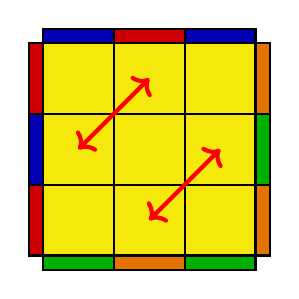
\begin{tikzpicture}[scale=0.9]
    % --- 1. Top Yellow Face (Solved) ---
    \foreach \x in {0,1,2} {
        \foreach \y in {0,1,2} {
            \path[top-y] (\x,\y) rectangle (\x+1,\y+1);
        }
    }

    % --- 2. Adjacent Side Stickers (Outer Ring) ---
    % BACK (Top edge of diagram - Blue face)
    \path[side-B] (0,3) rectangle (1,3.2);
    \path[side-R] (1,3) rectangle (2,3.2);
    \path[side-B] (2,3) rectangle (3,3.2);
    
    % FRONT (Bottom edge of diagram - Green face)
    \path[side-G] (0,-0.2) rectangle (1,0);
    \path[side-O] (1,-0.2) rectangle (2,0); % Scrambled Edge (Red)
    \path[side-G] (2,-0.2) rectangle (3,0);
    
    % LEFT (Left edge of diagram - Orange face)
    \path[side-R] (-0.2,0) rectangle (0,1);
    \path[side-B] (-0.2,1) rectangle (0,2); % Scrambled Edge (Green)
    \path[side-R] (-0.2,2) rectangle (0,3);
    
    % RIGHT (Right edge of diagram - Red face)
    \path[side-O] (3,0) rectangle (3.2,1);
    \path[side-G] (3,1) rectangle (3.2,2); % Scrambled Edge (Orange)
    \path[side-O] (3,2) rectangle (3.2,3);

    % --- 3. Permutation Arrows ---
    % Cycles edges: Front -> Left -> Right
    \draw[pllarrow,<->] (1.5, 0.5) -- (2.5, 1.5);
     \draw[pllarrow,<->] (0.5, 1.5) -- (1.5, 2.5);

\end{tikzpicture}

\medskip
\texttt{(M2' U M2' U) (M' U2) (M2' U2 M') [U2]}
\end{minipage}
\hfill
% ==================== CASE 4: H PERM ====================
\begin{minipage}{0.45\textwidth}
\centering
\subsubsection*{H-Permutation}
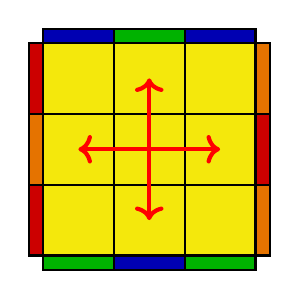
\begin{tikzpicture}[scale=0.9]
    % --- 1. Top Yellow Face (Solved) ---
    \foreach \x in {0,1,2} {
        \foreach \y in {0,1,2} {
            \path[top-y] (\x,\y) rectangle (\x+1,\y+1);
        }
    }

    % --- 2. Adjacent Side Stickers (Outer Ring) ---
    % BACK
    \path[side-B] (0,3) rectangle (1,3.2);
    \path[side-G] (1,3) rectangle (2,3.2);
    \path[side-B] (2,3) rectangle (3,3.2);
    
    % FRONT
    \path[side-G] (0,-0.2) rectangle (1,0); % Scrambled Corner (Orange)
    \path[side-B] (1,-0.2) rectangle (2,0);
    \path[side-G] (2,-0.2) rectangle (3,0);
    
    % LEFT
    \path[side-R] (-0.2,0) rectangle (0,1);
    \path[side-O] (-0.2,1) rectangle (0,2);
    \path[side-R] (-0.2,2) rectangle (0,3); % Scrambled Corner (Green)
    
    % RIGHT
    \path[side-O] (3,0) rectangle (3.2,1);
    \path[side-R] (3,1) rectangle (3.2,2); % Scrambled Edge (Blue)
    \path[side-O] (3,2) rectangle (3.2,3);

    % --- 3. Permutation Arrows ---
    % Swaps two right corners
    \draw[pllarrow, <->] (1.5, 0.5) -- (1.5, 2.5);
    % Swaps left and right edges
    \draw[pllarrow, <->] (0.5, 1.5) -- (2.5, 1.5);

\end{tikzpicture}

\medskip
\texttt{(M2' U M2') U2 (M2' U M2')}
\end{minipage}

% ==================== CASE 5: Aa PERM ====================
\begin{minipage}{0.45\textwidth}
\centering
\subsubsection*{Aa-Permutation}
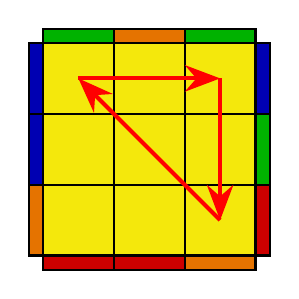
\begin{tikzpicture}[scale=0.9]
    % --- 1. Top Yellow Face (Solved) ---
    \foreach \x in {0,1,2} {
        \foreach \y in {0,1,2} {
            \path[top-y] (\x,\y) rectangle (\x+1,\y+1);
        }
    }

    % --- 2. Adjacent Side Stickers (Outer Ring) ---
    % BACK (Top edge of diagram - Blue face)
    \path[side-G] (0,3) rectangle (1,3.2);
    \path[side-O] (1,3) rectangle (2,3.2);
    \path[side-G] (2,3) rectangle (3,3.2);
    
    % FRONT (Bottom edge of diagram - Green face)
    \path[side-R] (0,-0.2) rectangle (1,0);
    \path[side-R] (1,-0.2) rectangle (2,0); % Scrambled Edge (Red)
    \path[side-O] (2,-0.2) rectangle (3,0);
    
    % LEFT (Left edge of diagram - Orange face)
    \path[side-O] (-0.2,0) rectangle (0,1);
    \path[side-B] (-0.2,1) rectangle (0,2); % Scrambled Edge (Green)
    \path[side-B] (-0.2,2) rectangle (0,3);
    
    % RIGHT (Right edge of diagram - Red face)
    \path[side-R] (3,0) rectangle (3.2,1);
    \path[side-G] (3,1) rectangle (3.2,2); % Scrambled Edge (Orange)
    \path[side-B] (3,2) rectangle (3.2,3);

    % --- 3. Permutation Arrows ---
    % Cycles edges: Front -> Left -> Right
    \draw[pllarrow] (0.5, 2.5) to (2.5, 2.5);
    \draw[pllarrow] (2.5, 2.5) to (2.5, 0.5);
    \draw[pllarrow] (2.5, 0.5) to (0.5, 2.5);

\end{tikzpicture}

\medskip
\texttt{x (R' U R') D2 (R U' R') D2 R2 x'}
\end{minipage}
\hfill
% ==================== CASE 6: Ab PERM ====================
\begin{minipage}{0.45\textwidth}
\centering
\subsubsection*{Ab-Permutation}
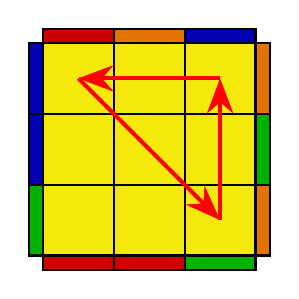
\begin{tikzpicture}[scale=0.9]
    % --- 1. Top Yellow Face (Solved) ---
    \foreach \x in {0,1,2} {
        \foreach \y in {0,1,2} {
            \path[top-y] (\x,\y) rectangle (\x+1,\y+1);
        }
    }

    % --- 2. Adjacent Side Stickers (Outer Ring) ---
    % BACK
    \path[side-R] (0,3) rectangle (1,3.2);
    \path[side-O] (1,3) rectangle (2,3.2);
    \path[side-B] (2,3) rectangle (3,3.2);
    
    % FRONT
    \path[side-R] (0,-0.2) rectangle (1,0); % Scrambled Corner (Orange)
    \path[side-R] (1,-0.2) rectangle (2,0);
    \path[side-G] (2,-0.2) rectangle (3,0);
    
    % LEFT
    \path[side-G] (-0.2,0) rectangle (0,1);
    \path[side-B] (-0.2,1) rectangle (0,2);
    \path[side-B] (-0.2,2) rectangle (0,3); % Scrambled Corner (Green)
    
    % RIGHT
    \path[side-O] (3,0) rectangle (3.2,1);
    \path[side-G] (3,1) rectangle (3.2,2); % Scrambled Edge (Blue)
    \path[side-O] (3,2) rectangle (3.2,3);

    % --- 3. Permutation Arrows ---
   \draw[pllarrow] (0.5, 2.5) to (2.5, 0.5);
    \draw[pllarrow] (2.5, 0.5) to (2.5, 2.5);
    \draw[pllarrow] (2.5, 2.5) to (0.5, 2.5);

\end{tikzpicture}

\medskip
\texttt{x R2' D2 (R U R') D2 (R U' R) x'}
\end{minipage}

% ==================== CASE 7: E PERM ====================
\begin{minipage}{0.45\textwidth}
\centering
\subsubsection*{E-Permutation}
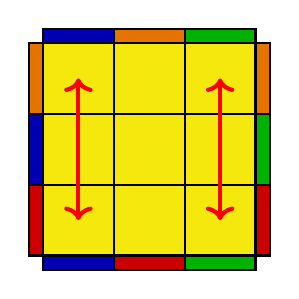
\begin{tikzpicture}[scale=0.9]
    % --- 1. Top Yellow Face (Solved) ---
    \foreach \x in {0,1,2} {
        \foreach \y in {0,1,2} {
            \path[top-y] (\x,\y) rectangle (\x+1,\y+1);
        }
    }

    % --- 2. Adjacent Side Stickers (Outer Ring) ---
    % BACK (Top edge of diagram - Blue face)
    \path[side-B] (0,3) rectangle (1,3.2);
    \path[side-O] (1,3) rectangle (2,3.2);
    \path[side-G] (2,3) rectangle (3,3.2);
    
    % FRONT (Bottom edge of diagram - Green face)
    \path[side-B] (0,-0.2) rectangle (1,0);
    \path[side-R] (1,-0.2) rectangle (2,0); % Scrambled Edge (Red)
    \path[side-G] (2,-0.2) rectangle (3,0);
    
    % LEFT (Left edge of diagram - Orange face)
    \path[side-R] (-0.2,0) rectangle (0,1);
    \path[side-B] (-0.2,1) rectangle (0,2); % Scrambled Edge (Green)
    \path[side-O] (-0.2,2) rectangle (0,3);
    
    % RIGHT (Right edge of diagram - Red face)
    \path[side-R] (3,0) rectangle (3.2,1);
    \path[side-G] (3,1) rectangle (3.2,2); % Scrambled Edge (Orange)
    \path[side-O] (3,2) rectangle (3.2,3);

    % --- 3. Permutation Arrows ---
    % Cycles edges: Front -> Left -> Right
    \   \draw[pllarrow,<->] (0.5, 0.5) -- (0.5, 2.5);
     \draw[pllarrow,<->] (2.5, 0.5) -- (2.5, 2.5);

\end{tikzpicture}

\medskip
\texttt{x (R' U R') D2 (R U' R') D2 R2 x'}
\end{minipage}
\hfill


% ==================== CASE 8: Ra PERM ====================
\begin{minipage}{0.45\textwidth}
\centering
\subsubsection*{Ra-Permutation}
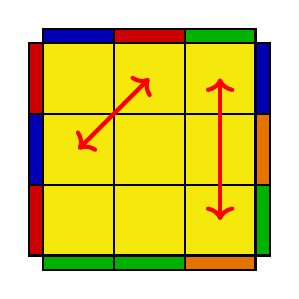
\begin{tikzpicture}[scale=0.9]
    % --- 1. Top Yellow Face (Solved) ---
    \foreach \x in {0,1,2} {
        \foreach \y in {0,1,2} {
            \path[top-y] (\x,\y) rectangle (\x+1,\y+1);
        }
    }

    % --- 2. Adjacent Side Stickers (Outer Ring) ---
    % BACK (Top edge of diagram - Blue face)
    \path[side-B] (0,3) rectangle (1,3.2);
    \path[side-R] (1,3) rectangle (2,3.2);
    \path[side-G] (2,3) rectangle (3,3.2);
    
    % FRONT (Bottom edge of diagram - Green face)
    \path[side-G] (0,-0.2) rectangle (1,0);
    \path[side-G] (1,-0.2) rectangle (2,0); % Scrambled Edge (Red)
    \path[side-O] (2,-0.2) rectangle (3,0);
    
    % LEFT (Left edge of diagram - Orange face)
    \path[side-R] (-0.2,0) rectangle (0,1);
    \path[side-B] (-0.2,1) rectangle (0,2); % Scrambled Edge (Green)
    \path[side-R] (-0.2,2) rectangle (0,3);
    
    % RIGHT (Right edge of diagram - Red face)
    \path[side-G] (3,0) rectangle (3.2,1);
    \path[side-O] (3,1) rectangle (3.2,2); % Scrambled Edge (Orange)
    \path[side-B] (3,2) rectangle (3.2,3);

    % --- 3. Permutation Arrows ---
    % Cycles edges: Front -> Left -> Right
    \draw[pllarrow,<->] (1.5, 2.5) -- (0.5, 1.5);
     \draw[pllarrow,<->] (2.5, 0.5) -- (2.5, 2.5);

\end{tikzpicture}

\medskip
\texttt{(R U' R' U') (R U R D) (R' U' R D') (R' U2 R') [U']}
\end{minipage}
\hfill
% ==================== CASE 9: Rb PERM ====================
\begin{minipage}{0.45\textwidth}
\centering
\subsubsection*{Rb-Permutation}
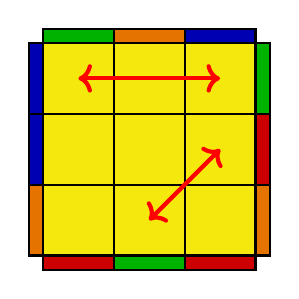
\begin{tikzpicture}[scale=0.9]
    % --- 1. Top Yellow Face (Solved) ---
    \foreach \x in {0,1,2} {
        \foreach \y in {0,1,2} {
            \path[top-y] (\x,\y) rectangle (\x+1,\y+1);
        }
    }

    % --- 2. Adjacent Side Stickers (Outer Ring) ---
    % BACK
    \path[side-G] (0,3) rectangle (1,3.2);
    \path[side-O] (1,3) rectangle (2,3.2);
    \path[side-B] (2,3) rectangle (3,3.2);
    
    % FRONT
    \path[side-R] (0,-0.2) rectangle (1,0); % Scrambled Corner (Orange)
    \path[side-G] (1,-0.2) rectangle (2,0);
    \path[side-R] (2,-0.2) rectangle (3,0);
    
    % LEFT
    \path[side-O] (-0.2,0) rectangle (0,1);
    \path[side-B] (-0.2,1) rectangle (0,2);
    \path[side-B] (-0.2,2) rectangle (0,3); % Scrambled Corner (Green)
    
    % RIGHT
    \path[side-O] (3,0) rectangle (3.2,1);
    \path[side-R] (3,1) rectangle (3.2,2); % Scrambled Edge (Blue)
    \path[side-G] (3,2) rectangle (3.2,3);

    % --- 3. Permutation Arrows ---
    \draw[pllarrow,<->] (1.5, 0.5) -- (2.5, 1.5);
     \draw[pllarrow,<->] (0.5, 2.5) -- (2.5, 2.5);
\end{tikzpicture}

\medskip
\texttt{(R' U2 R U2') R' F (R U R' U') R' F' R2 [U']}
\end{minipage}
\hfill

% ==================== CASE 10: Ja PERM ====================
\begin{minipage}{0.45\textwidth}
\centering
\subsubsection*{Ja-Permutation}
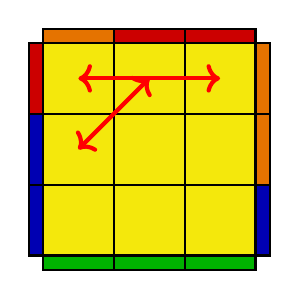
\begin{tikzpicture}[scale=0.9]
    % --- 1. Top Yellow Face (Solved) ---
    \foreach \x in {0,1,2} {
        \foreach \y in {0,1,2} {
            \path[top-y] (\x,\y) rectangle (\x+1,\y+1);
        }
    }

    % --- 2. Adjacent Side Stickers (Outer Ring) ---
    % BACK (Top edge of diagram - Blue face)
    \path[side-O] (0,3) rectangle (1,3.2);
    \path[side-R] (1,3) rectangle (2,3.2);
    \path[side-R] (2,3) rectangle (3,3.2);
    
    % FRONT (Bottom edge of diagram - Green face)
    \path[side-G] (0,-0.2) rectangle (1,0);
    \path[side-G] (1,-0.2) rectangle (2,0); % Scrambled Edge (Red)
    \path[side-G] (2,-0.2) rectangle (3,0);
    
    % LEFT (Left edge of diagram - Orange face)
    \path[side-B] (-0.2,0) rectangle (0,1);
    \path[side-B] (-0.2,1) rectangle (0,2); % Scrambled Edge (Green)
    \path[side-R] (-0.2,2) rectangle (0,3);
    
    % RIGHT (Right edge of diagram - Red face)
    \path[side-B] (3,0) rectangle (3.2,1);
    \path[side-O] (3,1) rectangle (3.2,2); % Scrambled Edge (Orange)
    \path[side-O] (3,2) rectangle (3.2,3);

    % --- 3. Permutation Arrows ---
    % Cycles edges: Front -> Left -> Right
    \draw[pllarrow,<->] (1.5, 2.5) -- (0.5, 1.5);
     \draw[pllarrow,<->] (0.5, 2.5) -- (2.5, 2.5);

\end{tikzpicture}

\medskip
\texttt{(R' U L' U2) (R U' R' U2 R) L [U']}
\end{minipage}
\hfill
% ==================== CASE 11: Jb PERM ====================
\begin{minipage}{0.45\textwidth}
\centering
\subsubsection*{Jb-Permutation}
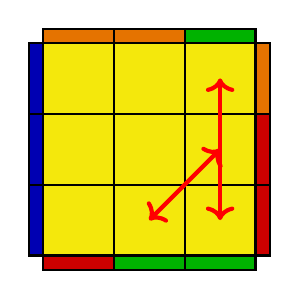
\begin{tikzpicture}[scale=0.9]
    % --- 1. Top Yellow Face (Solved) ---
    \foreach \x in {0,1,2} {
        \foreach \y in {0,1,2} {
            \path[top-y] (\x,\y) rectangle (\x+1,\y+1);
        }
    }

    % --- 2. Adjacent Side Stickers (Outer Ring) ---
    % BACK
    \path[side-O] (0,3) rectangle (1,3.2);
    \path[side-O] (1,3) rectangle (2,3.2);
    \path[side-G] (2,3) rectangle (3,3.2);
    
    % FRONT
    \path[side-R] (0,-0.2) rectangle (1,0); % Scrambled Corner (Orange)
    \path[side-G] (1,-0.2) rectangle (2,0);
    \path[side-G] (2,-0.2) rectangle (3,0);
    
    % LEFT
    \path[side-B] (-0.2,0) rectangle (0,1);
    \path[side-B] (-0.2,1) rectangle (0,2);
    \path[side-B] (-0.2,2) rectangle (0,3); % Scrambled Corner (Green)
    
    % RIGHT
    \path[side-R] (3,0) rectangle (3.2,1);
    \path[side-R] (3,1) rectangle (3.2,2); % Scrambled Edge (Blue)
    \path[side-O] (3,2) rectangle (3.2,3);

    % --- 3. Permutation Arrows ---
    \draw[pllarrow,<->] (1.5, 0.5) -- (2.5, 1.5);
     \draw[pllarrow,<->] (2.5, 0.5) -- (2.5, 2.5);
\end{tikzpicture}

\medskip
\texttt{(R U R' F') (R U R' U') R' F R2 U' R' [U']}
\end{minipage}
\hfill

% ==================== CASE 12: T PERM ====================
\begin{minipage}{0.45\textwidth}
\centering
\subsubsection*{T-Permutation}
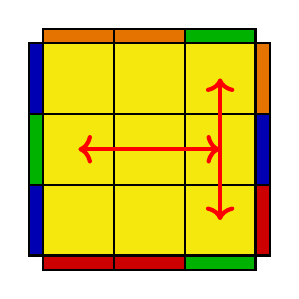
\begin{tikzpicture}[scale=0.9]
    % --- 1. Top Yellow Face (Solved) ---
    \foreach \x in {0,1,2} {
        \foreach \y in {0,1,2} {
            \path[top-y] (\x,\y) rectangle (\x+1,\y+1);
        }
    }

    % --- 2. Adjacent Side Stickers (Outer Ring) ---
    % BACK (Top edge of diagram - Blue face)
    \path[side-O] (0,3) rectangle (1,3.2);
    \path[side-O] (1,3) rectangle (2,3.2);
    \path[side-G] (2,3) rectangle (3,3.2);
    
    % FRONT (Bottom edge of diagram - Green face)
    \path[side-R] (0,-0.2) rectangle (1,0);
    \path[side-R] (1,-0.2) rectangle (2,0); % Scrambled Edge (Red)
    \path[side-G] (2,-0.2) rectangle (3,0);
    
    % LEFT (Left edge of diagram - Orange face)
    \path[side-B] (-0.2,0) rectangle (0,1);
    \path[side-G] (-0.2,1) rectangle (0,2); % Scrambled Edge (Green)
    \path[side-B] (-0.2,2) rectangle (0,3);
    
    % RIGHT (Right edge of diagram - Red face)
    \path[side-R] (3,0) rectangle (3.2,1);
    \path[side-B] (3,1) rectangle (3.2,2); % Scrambled Edge (Orange)
    \path[side-O] (3,2) rectangle (3.2,3);

    % --- 3. Permutation Arrows ---
    % Cycles edges: Front -> Left -> Right
    \draw[pllarrow,<->] (2.5, 2.5) -- (2.5, 0.5);
     \draw[pllarrow,<->] (0.5, 1.5) -- (2.5, 1.5);

\end{tikzpicture}

\medskip
\texttt{(R U R' U') (R' F R2 U') R' U' (R U R' F')}
\end{minipage}
\hfill
% ==================== CASE 13: F PERM ====================
\begin{minipage}{0.45\textwidth}
\centering
\subsubsection*{F-Permutation}
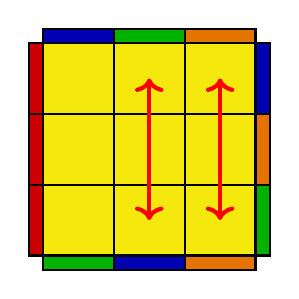
\begin{tikzpicture}[scale=0.9]
    % --- 1. Top Yellow Face (Solved) ---
    \foreach \x in {0,1,2} {
        \foreach \y in {0,1,2} {
            \path[top-y] (\x,\y) rectangle (\x+1,\y+1);
        }
    }

    % --- 2. Adjacent Side Stickers (Outer Ring) ---
    % BACK
    \path[side-B] (0,3) rectangle (1,3.2);
    \path[side-G] (1,3) rectangle (2,3.2);
    \path[side-O] (2,3) rectangle (3,3.2);
    
    % FRONT
    \path[side-G] (0,-0.2) rectangle (1,0); % Scrambled Corner (Orange)
    \path[side-B] (1,-0.2) rectangle (2,0);
    \path[side-O] (2,-0.2) rectangle (3,0);
    
    % LEFT
    \path[side-R] (-0.2,0) rectangle (0,1);
    \path[side-R] (-0.2,1) rectangle (0,2);
    \path[side-R] (-0.2,2) rectangle (0,3); % Scrambled Corner (Green)
    
    % RIGHT
    \path[side-G] (3,0) rectangle (3.2,1);
    \path[side-O] (3,1) rectangle (3.2,2); % Scrambled Edge (Blue)
    \path[side-B] (3,2) rectangle (3.2,3);

    % --- 3. Permutation Arrows ---
    \draw[pllarrow,<->] (1.5, 0.5) -- (1.5, 2.5);
     \draw[pllarrow,<->] (2.5, 0.5) -- (2.5, 2.5);
\end{tikzpicture}

\medskip
\texttt{(R' U' F')(R U R' U')(R' F R2 U')(R' U' R U)(R' U R)}
\end{minipage}
\hfill

% ==================== CASE 14: V PERM ====================
\begin{minipage}{0.45\textwidth}
\centering
\subsubsection*{V-Permutation}
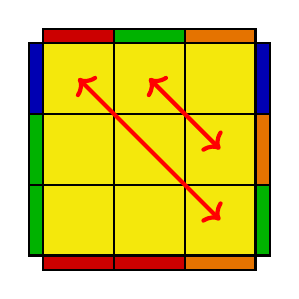
\begin{tikzpicture}[scale=0.9]
    % --- 1. Top Yellow Face (Solved) ---
    \foreach \x in {0,1,2} {
        \foreach \y in {0,1,2} {
            \path[top-y] (\x,\y) rectangle (\x+1,\y+1);
        }
    }

    % --- 2. Adjacent Side Stickers (Outer Ring) ---
    % BACK (Top edge of diagram - Blue face)
    \path[side-R] (0,3) rectangle (1,3.2);
    \path[side-G] (1,3) rectangle (2,3.2);
    \path[side-O] (2,3) rectangle (3,3.2);
    
    % FRONT (Bottom edge of diagram - Green face)
    \path[side-R] (0,-0.2) rectangle (1,0);
    \path[side-R] (1,-0.2) rectangle (2,0); % Scrambled Edge (Red)
    \path[side-O] (2,-0.2) rectangle (3,0);
    
    % LEFT (Left edge of diagram - Orange face)
    \path[side-G] (-0.2,0) rectangle (0,1);
    \path[side-G] (-0.2,1) rectangle (0,2); % Scrambled Edge (Green)
    \path[side-B] (-0.2,2) rectangle (0,3);
    
    % RIGHT (Right edge of diagram - Red face)
    \path[side-G] (3,0) rectangle (3.2,1);
    \path[side-O] (3,1) rectangle (3.2,2); % Scrambled Edge (Orange)
    \path[side-B] (3,2) rectangle (3.2,3);

    % --- 3. Permutation Arrows ---
    % Cycles edges: Front -> Left -> Right
    \draw[pllarrow,<->] (0.5, 2.5) -- (2.5, 0.5);
     \draw[pllarrow,<->] (1.5, 2.5) -- (2.5, 1.5);

\end{tikzpicture}

\medskip
\texttt{(R' U R' U') y (R' F' R2 U') (R' U R' F) R F}
\end{minipage}
\hfill
% ==================== CASE 15: Y PERM ====================
\begin{minipage}{0.45\textwidth}
\centering
\subsubsection*{Y-Permutation}
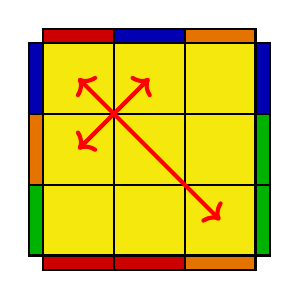
\begin{tikzpicture}[scale=0.9]
    % --- 1. Top Yellow Face (Solved) ---
    \foreach \x in {0,1,2} {
        \foreach \y in {0,1,2} {
            \path[top-y] (\x,\y) rectangle (\x+1,\y+1);
        }
    }

    % --- 2. Adjacent Side Stickers (Outer Ring) ---
    % BACK
    \path[side-R] (0,3) rectangle (1,3.2);
    \path[side-B] (1,3) rectangle (2,3.2);
    \path[side-O] (2,3) rectangle (3,3.2);
    
    % FRONT
    \path[side-R] (0,-0.2) rectangle (1,0); % Scrambled Corner (Orange)
    \path[side-R] (1,-0.2) rectangle (2,0);
    \path[side-O] (2,-0.2) rectangle (3,0);
    
    % LEFT
    \path[side-G] (-0.2,0) rectangle (0,1);
    \path[side-O] (-0.2,1) rectangle (0,2);
    \path[side-B] (-0.2,2) rectangle (0,3); % Scrambled Corner (Green)
    
    % RIGHT
    \path[side-G] (3,0) rectangle (3.2,1);
    \path[side-G] (3,1) rectangle (3.2,2); % Scrambled Edge (Blue)
    \path[side-B] (3,2) rectangle (3.2,3);

    % --- 3. Permutation Arrows ---
    \draw[pllarrow,<->] (0.5, 2.5) -- (2.5, 0.5);
     \draw[pllarrow,<->] (0.5, 1.5) -- (1.5, 2.5);
\end{tikzpicture}

\medskip
\texttt{F (R U' R' U') (R U R' F') (R U R' U') (R' F R F')}
\end{minipage}
\hfill

% ==================== CASE 16: Na PERM ====================
\begin{minipage}{0.45\textwidth}
\centering
\subsubsection*{Na-Permutation}
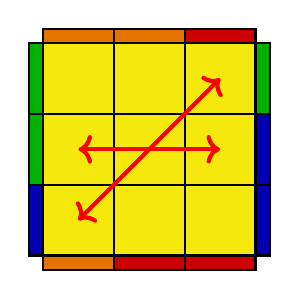
\begin{tikzpicture}[scale=0.9]
    % --- 1. Top Yellow Face (Solved) ---
    \foreach \x in {0,1,2} {
        \foreach \y in {0,1,2} {
            \path[top-y] (\x,\y) rectangle (\x+1,\y+1);
        }
    }

    % --- 2. Adjacent Side Stickers (Outer Ring) ---
    % BACK (Top edge of diagram - Blue face)
    \path[side-O] (0,3) rectangle (1,3.2);
    \path[side-O] (1,3) rectangle (2,3.2);
    \path[side-R] (2,3) rectangle (3,3.2);
    
    % FRONT (Bottom edge of diagram - Green face)
    \path[side-O] (0,-0.2) rectangle (1,0);
    \path[side-R] (1,-0.2) rectangle (2,0); % Scrambled Edge (Red)
    \path[side-R] (2,-0.2) rectangle (3,0);
    
    % LEFT (Left edge of diagram - Orange face)
    \path[side-B] (-0.2,0) rectangle (0,1);
    \path[side-G] (-0.2,1) rectangle (0,2); % Scrambled Edge (Green)
    \path[side-G] (-0.2,2) rectangle (0,3);
    
    % RIGHT (Right edge of diagram - Red face)
    \path[side-B] (3,0) rectangle (3.2,1);
    \path[side-B] (3,1) rectangle (3.2,2); % Scrambled Edge (Orange)
    \path[side-G] (3,2) rectangle (3.2,3);

    % --- 3. Permutation Arrows ---
    % Cycles edges: Front -> Left -> Right
    \draw[pllarrow,<->] (2.5, 2.5) -- (0.5, 0.5);
     \draw[pllarrow,<->] (0.5, 1.5) -- (2.5, 1.5);

\end{tikzpicture}

\medskip
\texttt{(R U R' U)(R U R' F')(R U R' U')(R' F R2 U') R' U2 (R U' R')}
\end{minipage}
\hfill
% ==================== CASE 17: Nb PERM ====================
\begin{minipage}{0.45\textwidth}
\centering
\subsubsection*{Nb-Permutation}
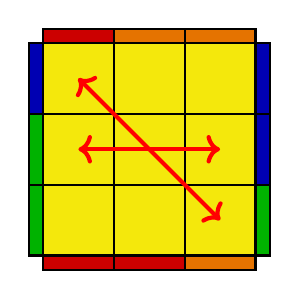
\begin{tikzpicture}[scale=0.9]
    % --- 1. Top Yellow Face (Solved) ---
    \foreach \x in {0,1,2} {
        \foreach \y in {0,1,2} {
            \path[top-y] (\x,\y) rectangle (\x+1,\y+1);
        }
    }

    % --- 2. Adjacent Side Stickers (Outer Ring) ---
    % BACK
    \path[side-R] (0,3) rectangle (1,3.2);
    \path[side-O] (1,3) rectangle (2,3.2);
    \path[side-O] (2,3) rectangle (3,3.2);
    
    % FRONT
    \path[side-R] (0,-0.2) rectangle (1,0); % Scrambled Corner (Orange)
    \path[side-R] (1,-0.2) rectangle (2,0);
    \path[side-O] (2,-0.2) rectangle (3,0);
    
    % LEFT
    \path[side-G] (-0.2,0) rectangle (0,1);
    \path[side-G] (-0.2,1) rectangle (0,2);
    \path[side-B] (-0.2,2) rectangle (0,3); % Scrambled Corner (Green)
    
    % RIGHT
    \path[side-G] (3,0) rectangle (3.2,1);
    \path[side-B] (3,1) rectangle (3.2,2); % Scrambled Edge (Blue)
    \path[side-B] (3,2) rectangle (3.2,3);

    % --- 3. Permutation Arrows ---
    \draw[pllarrow,<->] (0.5, 1.5) -- (2.5, 1.5);
     \draw[pllarrow,<->] (0.5, 2.5) -- (2.5, 0.5);
\end{tikzpicture}

\medskip
\texttt{(R' U R U') (R' F' U' F) (R U R' F) R' F' (R U' R)}
\end{minipage}
\hfill

% ==================== CASE 18: Ga PERM ====================
\begin{minipage}{0.45\textwidth}
\centering
\subsubsection*{Ga-Permutation}
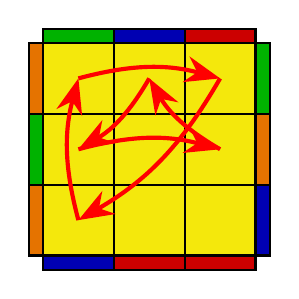
\begin{tikzpicture}[scale=0.9]
    % --- 1. Top Yellow Face (Solved) ---
    \foreach \x in {0,1,2} {
        \foreach \y in {0,1,2} {
            \path[top-y] (\x,\y) rectangle (\x+1,\y+1);
        }
    }

    % --- 2. Adjacent Side Stickers (Outer Ring) ---
    % BACK (Top edge of diagram - Blue face)
    \path[side-G] (0,3) rectangle (1,3.2);
    \path[side-B] (1,3) rectangle (2,3.2);
    \path[side-R] (2,3) rectangle (3,3.2);
    
    % FRONT (Bottom edge of diagram - Green face)
    \path[side-B] (0,-0.2) rectangle (1,0);
    \path[side-R] (1,-0.2) rectangle (2,0); % Scrambled Edge (Red)
    \path[side-R] (2,-0.2) rectangle (3,0);
    
    % LEFT (Left edge of diagram - Orange face)
    \path[side-O] (-0.2,0) rectangle (0,1);
    \path[side-G] (-0.2,1) rectangle (0,2); % Scrambled Edge (Green)
    \path[side-O] (-0.2,2) rectangle (0,3);
    
    % RIGHT (Right edge of diagram - Red face)
    \path[side-B] (3,0) rectangle (3.2,1);
    \path[side-O] (3,1) rectangle (3.2,2); % Scrambled Edge (Orange)
    \path[side-G] (3,2) rectangle (3.2,3);

    % --- 3. Permutation Arrows ---
    % Cycles edges: Front -> Left -> Right
    \draw[pllarrow] (0.5, 0.5) to[bend left=15] (0.5, 2.5);
    \draw[pllarrow] (0.5, 2.5) to[bend left=15] (2.5, 2.5);
    \draw[pllarrow] (2.5, 2.5) to[bend left=15] (0.5, 0.5);
     \draw[pllarrow] (0.5, 1.5) to[bend left=15] (2.5, 1.5);
    \draw[pllarrow] (2.5, 1.5) to[bend left=15] (1.5, 2.5);
    \draw[pllarrow] (1.5, 2.5) to[bend left=15] (0.5, 1.5);

\end{tikzpicture}

\medskip
\texttt{R2 U (R' U R' U') (R U' R2) D U' (R' U R D') [U]}
\end{minipage}
\hfill
% ==================== CASE 19: Gb PERM ====================
\begin{minipage}{0.45\textwidth}
\centering
\subsubsection*{Gb-Permutation}
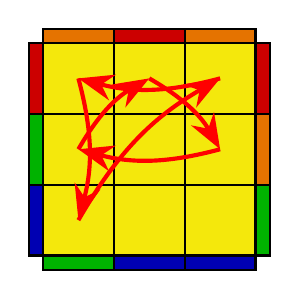
\begin{tikzpicture}[scale=0.9]
    % --- 1. Top Yellow Face (Solved) ---
    \foreach \x in {0,1,2} {
        \foreach \y in {0,1,2} {
            \path[top-y] (\x,\y) rectangle (\x+1,\y+1);
        }
    }

    % --- 2. Adjacent Side Stickers (Outer Ring) ---
    % BACK
    \path[side-O] (0,3) rectangle (1,3.2);
    \path[side-R] (1,3) rectangle (2,3.2);
    \path[side-O] (2,3) rectangle (3,3.2);
    
    % FRONT
    \path[side-G] (0,-0.2) rectangle (1,0); % Scrambled Corner (Orange)
    \path[side-B] (1,-0.2) rectangle (2,0);
    \path[side-B] (2,-0.2) rectangle (3,0);
    
    % LEFT
    \path[side-B] (-0.2,0) rectangle (0,1);
    \path[side-G] (-0.2,1) rectangle (0,2);
    \path[side-R] (-0.2,2) rectangle (0,3); % Scrambled Corner (Green)
    
    % RIGHT
    \path[side-G] (3,0) rectangle (3.2,1);
    \path[side-O] (3,1) rectangle (3.2,2); % Scrambled Edge (Blue)
    \path[side-R] (3,2) rectangle (3.2,3);

    % --- 3. Permutation Arrows ---
   \draw[pllarrow] (0.5, 0.5) to[bend left=15] (2.5, 2.5);
    \draw[pllarrow] (0.5, 2.5) to[bend left=15] (0.5, 0.5);
    \draw[pllarrow] (2.5, 2.5) to[bend left=15] (0.5, 2.5);
     \draw[pllarrow] (0.5, 1.5) to[bend left=15] (1.5, 2.5);
    \draw[pllarrow] (2.5, 1.5) to[bend left=15] (0.5, 1.5);
    \draw[pllarrow] (1.5, 2.5) to[bend left=15] (2.5, 1.5);
\end{tikzpicture}

\medskip
\texttt{(F' U' F) (R2 u R' U) (R U' R u') R2'}
\end{minipage}
\hfill

% ==================== CASE 20: Gc PERM ====================
\begin{minipage}{0.45\textwidth}
\centering
\subsubsection*{Gc-Permutation}
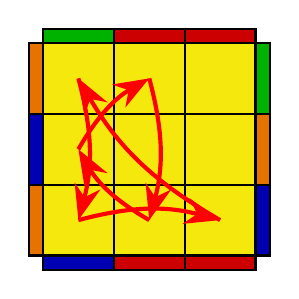
\begin{tikzpicture}[scale=0.9]
    % --- 1. Top Yellow Face (Solved) ---
    \foreach \x in {0,1,2} {
        \foreach \y in {0,1,2} {
            \path[top-y] (\x,\y) rectangle (\x+1,\y+1);
        }
    }

    % --- 2. Adjacent Side Stickers (Outer Ring) ---
    % BACK (Top edge of diagram - Blue face)
    \path[side-G] (0,3) rectangle (1,3.2);
    \path[side-R] (1,3) rectangle (2,3.2);
    \path[side-R] (2,3) rectangle (3,3.2);
    
    % FRONT (Bottom edge of diagram - Green face)
    \path[side-B] (0,-0.2) rectangle (1,0);
    \path[side-R] (1,-0.2) rectangle (2,0); % Scrambled Edge (Red)
    \path[side-R] (2,-0.2) rectangle (3,0);
    
    % LEFT (Left edge of diagram - Orange face)
    \path[side-O] (-0.2,0) rectangle (0,1);
    \path[side-B] (-0.2,1) rectangle (0,2); % Scrambled Edge (Green)
    \path[side-O] (-0.2,2) rectangle (0,3);
    
    % RIGHT (Right edge of diagram - Red face)
    \path[side-B] (3,0) rectangle (3.2,1);
    \path[side-O] (3,1) rectangle (3.2,2); % Scrambled Edge (Orange)
    \path[side-G] (3,2) rectangle (3.2,3);

    % --- 3. Permutation Arrows ---
    \draw[pllarrow] (0.5, 0.5) to[bend left=15] (2.5, 0.5);
    \draw[pllarrow] (0.5, 2.5) to[bend left=15] (0.5, 0.5);
    \draw[pllarrow] (2.5, 0.5) to[bend left=15] (0.5, 2.5);
     \draw[pllarrow] (0.5, 1.5) to[bend left=15] (1.5, 2.5);
    \draw[pllarrow] (1.5, 0.5) to[bend left=15] (0.5, 1.5);
    \draw[pllarrow] (1.5, 2.5) to[bend left=15] (1.5, 0.5);
\end{tikzpicture}

\medskip
\texttt{R2 U' (R U' R U) (R' U R2 D') (U R U' R') D [U']}
\end{minipage}
\hfill
% ==================== CASE 21: Gd PERM ====================
\begin{minipage}{0.45\textwidth}
\centering
\subsubsection*{Gd-Permutation}
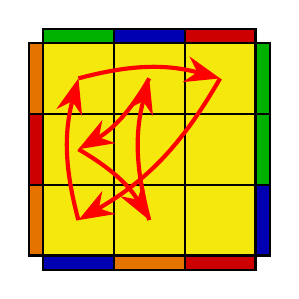
\begin{tikzpicture}[scale=0.9]
    % --- 1. Top Yellow Face (Solved) ---
    \foreach \x in {0,1,2} {
        \foreach \y in {0,1,2} {
            \path[top-y] (\x,\y) rectangle (\x+1,\y+1);
        }
    }

    % --- 2. Adjacent Side Stickers (Outer Ring) ---
    % BACK
    \path[side-G] (0,3) rectangle (1,3.2);
    \path[side-B] (1,3) rectangle (2,3.2);
    \path[side-R] (2,3) rectangle (3,3.2);
    
    % FRONT
    \path[side-B] (0,-0.2) rectangle (1,0); % Scrambled Corner (Orange)
    \path[side-O] (1,-0.2) rectangle (2,0);
    \path[side-R] (2,-0.2) rectangle (3,0);
    
    % LEFT
    \path[side-O] (-0.2,0) rectangle (0,1);
    \path[side-R] (-0.2,1) rectangle (0,2);
    \path[side-O] (-0.2,2) rectangle (0,3); % Scrambled Corner (Green)
    
    % RIGHT
    \path[side-B] (3,0) rectangle (3.2,1);
    \path[side-G] (3,1) rectangle (3.2,2); % Scrambled Edge (Blue)
    \path[side-G] (3,2) rectangle (3.2,3);

    % --- 3. Permutation Arrows ---
    \draw[pllarrow] (0.5, 0.5) to[bend left=15] (0.5, 2.5);
    \draw[pllarrow] (0.5, 2.5) to[bend left=15] (2.5, 2.5);
    \draw[pllarrow] (2.5, 2.5) to[bend left=15] (0.5, 0.5);
     \draw[pllarrow] (0.5, 1.5) to[bend left=15] (1.5, 0.5);
    \draw[pllarrow] (1.5, 2.5) to[bend left=15] (0.5, 1.5);
    \draw[pllarrow] (1.5, 0.5) to[bend left=15] (1.5, 2.5);
\end{tikzpicture}

\medskip
\texttt{D' (R U R' U') D (R2 U' R U') (R' U R' U) R2 [U]}
\end{minipage}
\hfill

\end{document}